\input{chapter-header.tex}
% =============================================================================
\chapter{Introduction}
\chaplabel{introduction}
\minitoc
% =============================================================================


%Reflective systems are those that reason about and act upon themselves \cite{Smit84a}. A causal connection exists between the program and its representation inside the program itself as a meta-program \cite{Maes87a}. This reflective architecture introduces self-references:  an object-oriented system is composed by objects, which are instances of classes, which are also objects, and so on. These self-references, also known as meta-circularities \cite{Chib96a}, allow the manipulation of several meta-levels on one infrastructure.
%
%Reflective systems traditionally modify their self-representation to evolve and define new abstractions. However, the self-modification approach of evolution has many drawbacks, such as making difficult the self-surgery operations~\cite{Casa09a} or the lose of the reproducibility of the system. On the other hand, non-reflective systems develop an evolution approach by recreation. Whenever a change has to be made to the system, a new system is created with the new changes applied. This approach solves many of the drawbacks of the reflective approach.
%
%\gp{add some sentences on why it is important to evolve, which kind of software artifacts we would like to evolve, why it is challenging}

% =============================================================================
%\section{The need for Software Evolution}
% =============================================================================

Software inevitable changes and we need to provide with the tools and methodologies that support such changes~\cite{Nier08b}. However, production-ready applications are not usually change-aware. These applications should be either engineered from scratch with change in mind, or a lot of reengineering effort should be invested in them to support change. Making deep modifications to a language runtime can be a cumbersome task.
At the same time, evolving a language runtime has become an important task in the last years. Multicore hardware brought new problems on concurrency and parallelism; the \emph{cloud} increased the need for software adaptation; new resource constrained devices such as phones are as current as almost every person has one in their our pockets. These new technologies present new challenges to software developers. The software we use, and in particular the programming languages and tools we use should be easily tailorable to support many of the new challenges that come with new technology and needs.

% =============================================================================
%\section{Resource Constrained Devices}
% =============================================================================

%\gp{noury had a reference on this -> everything is going small}

%Unused deployed code units have an undesired impact when targeting a constrained infrastructure. 
%Constrained devices may present restrictive hardware such as low primary or secondary memory, or even software impositions such as the Android's Dalvik VM restriction to deploy only 65536 methods\footnote{According to dalvik's bytecode documentation~(\url{http://source.android.com/devices/tech/dalvik/dalvik-bytecode.html}), the source register accepts values between 0 and 65536.}. Big JavaScript mashup applications have an impact on loading time due to network speed and parsing time.
%These limitations may forbid the deployment of applications that contain lots of code units, or limit the amount of applications and content an user can have in its device.

%Existing solutions to this problem propose the extraction of used code units of an application to reduce their size and memory footprint. Java Micro Edition~\cite{JavaME} proposes a general purpose specialized runtime environment with no possibility of customization. Other solutions in the field propose to automatically detect and extract used code units, so called \emph{tailoring}, with static call graph construction as the most dominant technique~\cite{ShortGrov97a}. 
%Static approaches present limitations in the presence of dynamic features such as reflection or in the absence of static type annotations. Additionally, these existing solutions are generally designed to extract all used code units with no possibility for the user to customize the process of selection.

For example, an application runtime should be easily tailorable to consume less resources. We can observe that deployed applications contain a set of \emph{code units} such as classes and methods that tend to occupy more memory~(primary and secondary) than necessary.
%Besides, an application may load a code unit that is only partially used, such as a class with some methods that are never invoked.
%Deployed object-oriented applications often contain \emph{code units}~(e.g. packages, classes, methods) that the running application never uses. 
This problem shows itself more evident and harder to control under the usage of third party software. 
Third party libraries and frameworks are designed in a generic fashion that allows multiple usages and functionalities, while applications use only few of them. 
Examples are logging libraries, web application frameworks or object-relational mappers.


%Figure~\ref{fig:unusedCodeUnits} shows a typical deployment scenario with unused code units.
%
%This problem becomes more evident with the inclusion of third party libraries~(and frameworks). 
%Third party libraries provide often a great variety of code units, usually designed in a generic fashion. 
%They allow multiple usages, while applications tend to use only some of them. 
%Additionally, application developers do not often modify and customize third party libraries to fit their needs but use them as black boxes. 
%Modifying them would mean to lose compatibility with the original development branch of the library and having deep knowledge on the library.
%
%\begin{figure}[ht]
%\begin{center}
%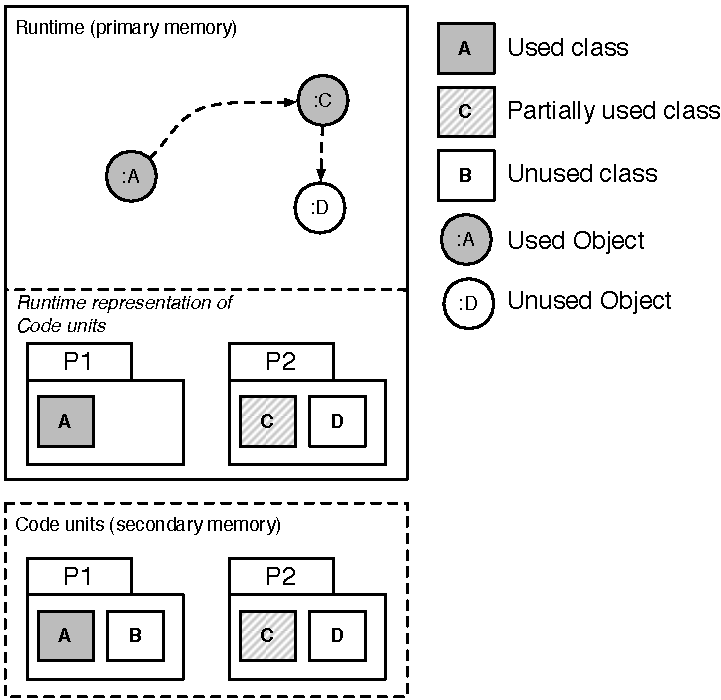
\includegraphics[width=1\linewidth]{components}
%\caption{\textbf{Unused Code Units.} Package P1 contains class A which is used during runtime and class B which is never needed and thus, not loaded. Package P2 contains class C which is partially used~(it contains methods that are never invoked) though it's completely loaded. Class D is loaded because an instance of it is created, but it is never used.\label{fig:unusedCodeUnits}}
%\end{center}
%\end{figure}

Unused code units represent serious drawbacks in constrained devices. 
First, unused code units may forbid the deployment into a constrained resource device.
It may also interfere with the deployment and usage of other applications, because of large memory footprints in both secondary~(disk storage) and primary~(RAM) memory~\cite{Mart12a} or the presence of slow networks in the case of rich web applications.
Second, some deployment targets may have an infrastructure designed in such a manner that forbids the deployment of large applications. For example, the Android's Dalvik VM restricts an application to deploy only 65536 methods.


% =============================================================================
%\section{The cloud and Mobile code}
% =============================================================================

%\gp{explain why code mobility is important!}

Another example of support that should be brought to user applications is \emph{code mobility}. Code mobility is a mechanism that allows the migration of programs between different environments. This problem is important in the context of ubiquitous systems and virtualization technology. Code mobility provides support for \eg load balancing, adjusting an application's resources dynamically and functionality customization. Fuggetta et al. define informally code mobility as the capability to rebind a piece of code with the location it is running~\cite{Fugg98a}. The languages and applications we develop should support this kind of rebinding and, more generally, be adaptable to new situations.

To answer these questions we propose \Vtt: a language virtualization infrastructure. With \Vtt we can virtualize a language runtime for its control and manipulation. This manipulation is transparent for the virtualized runtime. We show how \Vtt simplifies two different language runtime evolution paths: the language recreation by bootstrapping and the application extraction to reduce its memory consumption.

% =============================================================================
\section{What to Evolve?}
% =============================================================================

In the context of evolution of language and applications, we ask ourselves the following question: \emph{What are the elements of programming languages we should focus on?} High-level language runtimes are inherent complex pieces of software.
First, high-level languages virtual machines~(\VMs) have to combine two rather extreme goals: abstraction and performance.
We have seen that the required abstraction for the running high-level language has a strong influence on the \VM design.
At the same time the hard performance requirement requires precise interaction with the underlying hardware.
This goes even so far that specialized hardware is conceived to match the performance requirements \cite{Unga84a,Stef84a,McGh98a,Clic05a}.


On top of these complex \VMs, we run our  languages and applications.
These programs must comply to the contract required by the \VM to run, namely the \VM's \emph{execution model}.
A \VM's execution model imposes for example an object format, a class or prototype model to perform a method lookup, a bytecode set to execute methods at runtime.
In some cases, the \VM also loads and initializes the language structures.
These \VM-language complex interactions makes difficult to evolve any of these elements without affecting the other.

In the following sections we propose a dissection of a high-level program that runs on a \VM. We made this dissection with the objective of understanding the relation and separation between the elements we believe important in the context of software and language evolution. These sections do also state the terminology used during the rest of this dissertation. Figure \ref{fig:whatToEvolve} shows an schema of this dissection.

\begin{figure}[!ht]
\begin{center}
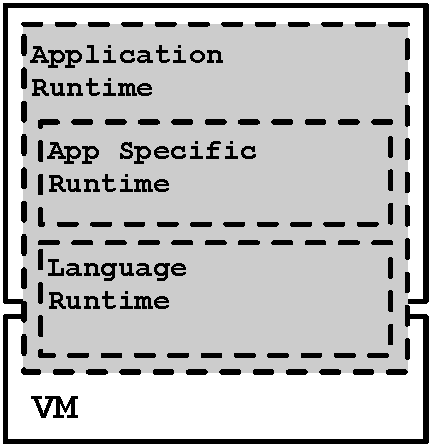
\includegraphics[width=0.6\linewidth]{elements_to_evolve}
\caption{\textbf{What to Evolve.}\label{fig:whatToEvolve}}
\end{center}
\end{figure}



\subsection{Virtual Machines}

\VMs concentrate several complex and interconnected elements with two main purposes: first it is to abstract applications from details such as memory management or machine specifics; second is to do that while also obtaining good performance.
The early \VMs focused on interpreting an abstract instruction set (bytecodes).
The benefits are twofold.
On the one hand the bytecodes guarantee certain platform independence by abstracting away from the \CPU specific instruction set.
On the other hand bytecodes allow to encode complex operations into little space both serving the hard memory constraints of the hardware and simplifying the design of a compiler.
Obviously this abstraction gain comes at a cost and ever since the first \VMs were built research and industry strive to reduce the interpretation overhead.

An efficient way to improve performance is to use a just in time compiler (\JIT) that dynamically generates native code from the bytecode \cite{Deut84a}.
In this case the bytecode becomes an intermediate representation (\IR) for a bigger compiler infrastructure.
However, \JIT compilers are notoriously complex as they crosscut many \VM components.
At the same time they crosscut all abstraction layers; they have to access high-level information from the running bytecodes and manage native code at the same time.
Similar complexity applies to the automatic memory management present in most high-level language \VMs.
Garbage Collectors (\GC) evolved from simple helpers to complex software artifacts that for instance support concurrent garbage collection \cite{Clic05a}.

In this context, being able to evolve a \VM is crucial for language evolution, as \VMs are the enablers of many of the features in programming languages. A \VM complexity should be engineered to favor its change. In this thesis we do not focus on \VM evolution but on the languages and applications that run of top of them. However, we have \VMs in mind as they are very interlaced with the languages we want to evolve and they impose and constraint our languages to their execution model.

\subsection{Application Runtime}

The application runtime is the set of elements that an application includes at runtime \eg libraries, objects, classes, methods. The \VM interprets and executes the application runtime. Indeed, with this purpose the application runtime must comply to the \VM execution model~(Figure \ref{fig:whatToEvolve}).

The \emph{language runtime} is the subset of the application runtime that describe the concepts and behavior available in the language we use \ie the set of classes, methods and constructs that describe the language internals. The language runtime concretizes the model that the language proposes to the developers. For example, Pharo Smalltalk proposes a programming model of classes with metaclasses~(the class of a class). This programming model is implemented in Pharo with the concrete existence of the \ct{Class} and \ct{Metaclass} classes and the implicit creation of a metaclass for each class we create. Additionally, a language runtime is not only composed by classes but also by other objects. For example, it contains a table of interned strings or \emph{symbols} that should be guaranteed unique in the system.

While indeed an application runtime~(and therefore its language runtime) is coupled to its \VM to run, sometimes it is also coupled in its definition. That is, the \VM defines and fixes the language model and some of the initially loaded libraries. In this context, we focus on the evolution of application runtimes. We would like to extend or specialize an application runtime by (a) modifying the concepts provided by the language and (b) adapt existing programs to new situations.

\section{Problem Statement}

\gp{I don't know where to put this yet}

\section{Contributions}

The contributions of this thesis are three-fold. First we describe \Vtt, an \emph{infrastructure for application runtime virtualization}. This infrastructure allows us to modify and control the virtualized application's runtime.
Second, we describe the process to create a language runtime through \emph{bootstrapping}. \Vtt provides this bootstrapping process with a clear interface  to manipulate the language and to use the tools and abstractions of the high-level language for its own creation.
Finally, we introduce an \emph{application extraction mechanism} based on lazy installation, namely Run-Fail-Grow~(RFG). \Vtt supports RFG by allowing the monitoring of the application under extraction and provide with facilities for code installation.

% =============================================================================
\section{Thesis Outline}
% =============================================================================
%\sm{This dissertation structure is different to what I am used to. At least the way you announce the purpose of the chapters is not what I would expect.
%In my diss, everything revolves around one thesis, here, it is a number of things listed one after another, don't see the central motive I would expect}

\gp{write from scratch, left for the end}
\begin{description}
\item[\chapref{background}] sheds light on the context of this work.
	We present a quick overview of language-side reflection followed by a development of \VM-level reflection.
	We find that mostly metacircular \VMs provide limited \VM-level reflection and thus we present several high-level language \VMs falling into this category.
	We conclude that there is only two research \VM that has a uniform model for \VM and language-side.
	Among them is \P a research \ST \VM we contributed to previous to working on this dissertation.

%\item[\chapref{reification}] focuses on language-side applications that simplify the interaction with the underlying \VM.
%	We present a custom inspector framework that is now used by default in \PH.
%	As a second part we explain how we introduced first-class layouts and slots to \PH to reify the low-level structural layout of objects.
%	Both projects are crucial for metacircular \VM development and are direct results from the research conducted on the \P \VM.

\item[\chapref{benzo}] describes a high-level low-level programming framework named \B.
	The core functionality of \B is to dynamically execute native-code generated at language-side.
	\B allows us to hoist typical \VM plugins to the language-side.
	Furthermore we show how code caching makes \B efficient and users essentially only pay a one-time overhead for generating the native code.
	
\item[\chapref{ffi}] presents \NB, a stable foreign function interface (\FFI) implementation that is entirely written at language-side using \B.
	\NB is a real-world validation of \B as it combines both language-side flexibility with \VM-level performance.
	We show in detail how \NB outperforms other existing \FFI solutions on \PH.

\item[\chapref{validation}] focuses on two further \B applications.
	In the first part we present \WF a framework for dynamically generating primitives at runtime.
	\WF extends the concept of metacircularity to the running language by reusing the same sources for dynamic primitives that were previously used to generate the static \VM artifact.
	In a first validation we show how \WF outperforms other reflective language-side solutions to instrument primitives.
	
	In a second part of \chapref{validation} we present \NBJ a prototype \JIT compiler that is based on \B.
	\NBJ shows the limitations of the \B approach as it required a customized \VM to communicate with the existing \JIT interface for native code.
	Our prototype implementation generates the same native code as the existing \VM-level \JIT, however, it is currently limited to simple expressions.
	\NBJ shows that for certain applications a well-define interface with the low-level components of the \VM is required.

\item[\chapref{future}] summarizes the limitations of \B and its application.
Furthermore we list undergoing efforts on the \B infrastructure and future work.

\item[\chapref{conclusion}] concludes the dissertation.

\end{description}


% =============================================================================
\input{chapter-footer.tex}
% =============================================================================